% !TEX program = XeLaTeXmk
% !TeX root = Babelfish.tex
% !TEX program = XeLaTeXmk
\documentclass[paper=a4,titlepage,english]{scrreprt}
\usepackage[olines,footsepline]{scrpage2}
\usepackage{scrhack}
\usepackage{amssymb} % before fontspec
\usepackage{xcolor,graphicx}
\usepackage{fontspec}
\usepackage{xltxtra}
\defaultfontfeatures{Mapping=tex-text}
%\setmonofont[Scale=1.02]{Consolas}
%\setmainfont{Georgia}
%\setsansfont{Univers LT 45 Light}
\usepackage{babel}
\usepackage{draftwatermark}
\SetWatermarkLightness{0.9}
\usepackage[marginal]{footmisc}
\usepackage{booktabs}
\usepackage{abstract}
\usepackage{tabularx}
\usepackage[rounded]{syntax}
\usepackage{float}
\usepackage{enumerate}
\setcounter{tocdepth}{2}
\setcounter{secnumdepth}{3}
\usepackage[final]{listings}
\usepackage[footnotesize,format=hang,justification=centering,singlelinecheck=off,nooneline]{caption}
\DeclareCaptionLabelFormat{continued}{#1~#2~(cont.)}
\captionsetup[ContinuedFloat]{labelformat=continued}
\usepackage{tikz}
\usetikzlibrary{shapes,arrows,positioning}

\usepackage[tikz]{bclogo}
\makeatletter
\@namedef{Gin@rule@.mps}#1{{eps}{.mps}{#1}}
\def\Gin@extensions{.pdf,.eps,.ps,.png,.jpg,.bmp,.pict,.tif,.psd,.mac,.sga,.tga,.gif,.mps}
\makeatother
\newcommand{\detail}[2][]{\begin{bclogo}[logo=\bcloupe, couleurBarre=gray,noborder=true,sousTitre={#1}]{Detail}#2\end{bclogo}}
\newcommand{\info}[2][]{\begin{bclogo}[logo=\bcinfo, couleurBarre=yellow,noborder=true,sousTitre={#1}]{Info}#2\end{bclogo}}
\newcommand{\att}[2][]{\begin{bclogo}[logo=\bcattention, couleurBarre=orange,noborder=true,sousTitre={#1}]{Warning}#2\end{bclogo}}
\newcommand{\warn}[2][]{\begin{bclogo}[logo=\bcdanger, couleurBarre=red,noborder=true,sousTitre={#1}]{Danger}#2\end{bclogo}}

\lstdefinelanguage{scala}{
  morekeywords={abstract,case,catch,class,def,
    do,else,extends,false,final,finally,
    for,if,implicit,import,match,mixin,
    new,null,object,override,package,
    private,protected,requires,return,sealed,
    super,this,throw,trait,true,try,
    type,val,var,while,with,yield},
  otherkeywords={=>,<-,<\%,<:,>:,\#,@},
  sensitive=true,
  morecomment=[l]{//},
  morecomment=[n]{/*}{*/},
  morestring=[b]",
%  morestring=[b]',
  morestring=[b]"""
}
\lstset{
  captionpos=b,
  columns=fullflexible,
  showspaces=false,
  showstringspaces=false,
  keepspaces,
  upquote=true,
  language=scala,
  basicstyle=\small\ttfamily,
  literate={~}{$\sim$}{1},
  backgroundcolor=\color{black!20}
}
\usepackage[
	unicode,
	pdfencoding=auto,
	pdftitle={Babelfish - A Graph-Based Data Warehouse},
	pdfauthor={Raphael Schweizer, Daniel Kröni, Remo Gisi},
	pdfsubject={Babelfish - Technical Documentation},
	pdfcreator={XeLaTeX},
%	pdfpagemode=FullScreen,
	colorlinks=true,
	linkcolor=black,
	hyperindex=true,
	urlcolor=black,
	citecolor=black,
	pdfdisplaydoctitle=true,
	pdfkeywords={}
	]{hyperref}

% glossaries options: section=section,numberedsection=nolabel,numberline
\usepackage[toc,acronym,nonumberlist,nolong,nosuper,notree,xindy]{glossaries} % load after hyperref
\renewcommand{\glspostdescription}{} % no '.' after description

\newcommand{\todo}[1][]{\textcolor{red}{\textbf{TODO} #1}}
\newcommand{\tbd}[1][]{\textcolor{red}{\textbf{TBD} #1}}
\newcommand\code[1]{\texttt{\hyphenchar\font45\relax #1}} %45 for -, 46 for .
\newcommand\abs[1]{\left|#1\right|}
\newcommand\norm[2]{\left\|#2\right\|_#1}
\usepackage{xparse}
\NewDocumentCommand\sbs{O{0.4}O{0.4}mm}{\begin{minipage}{#1\linewidth}#3\end{minipage}\hfill\begin{minipage}{#2\linewidth}#4\end{minipage}}

\newcommand{\fhnw}{
\includegraphics{FHNW}}
\newcommand{\texttth}[1]{\texttt{\hyphenchar\font45\relax #1}}
\newcommand{\frontmatter}{
	\clearpage
	\pagenumbering{roman}
	\refoot[]{\vspace{-1em}\normalfont\pagemark}
	\rofoot[]{\vspace{-1em}\normalfont\pagemark}
}
\newcommand{\mainmatter}{
 \clearpage
 \pagenumbering{arabic}
 \refoot[]{\vspace{-1em}\normalfont\pagemark}
 \rofoot[]{\vspace{-1em}\normalfont\pagemark}
}
\newcommand{\backmatter}{
 \clearpage
 \pagenumbering{Roman}
}

\usepackage{chngcntr}
\counterwithout{footnote}{chapter}
\usepackage{cleveref}

\setlength{\parindent}{0em}
\setlength{\parskip}{0.2\baselineskip}
\setlength{\topmargin}{-24mm}
\setlength{\topskip}{6mm}
\setlength{\footskip}{1cm}
\setlength{\skip\footins}{8mm}
\setlength{\footnotemargin}{0em}
%\setlength{\footnotesep}{0.3cm}
\setlength{\evensidemargin}{+3.6mm} % rel. to 1-inch / 2.54cm default
\setlength{\oddsidemargin}{+3.6mm}
\setlength{\textwidth}{15.2cm}
\setlength{\textheight}{24.5cm}
\setlength{\headheight}{2cm}
\setlength{\abovecaptionskip}{0.3cm}

\pagestyle{scrheadings}
% normal pagestyle also for chapter pages
%\renewcommand*{\chapterpagestyle}{scrheadings}
%\renewcommand*{\chapterheadstartvskip}{\vspace*{-\topskip}}
\setheadwidth[-7mm]{text}
\lohead[\fhnw]{\fhnw}
\lehead[\fhnw]{\fhnw}
\rohead{}
\rehead{}
\chead{}

\lefoot[]{\vspace{-1em}\normalfont Babelfish}
\lofoot[]{\vspace{-1em}\normalfont Babelfish}
\refoot[]{\vspace{-1em}\normalfont\pagemark}
\rofoot[]{\vspace{-1em}\normalfont\pagemark}
\cfoot[]{\vspace{-1em}\normalfont Documentation}

\makeatletter
\def\maketitle{
 \thispagestyle{plain}
 \pagenumbering{Alph}
 \null
 \vfill
 {\noindent \Huge \sffamily \textbf \@title\par}
 \vspace{1cm}
 {\noindent \LARGE \sffamily \textbf \@subtitle\par}
 \vspace{1cm}
 {\noindent \@date}
 \vfill
 \begin{table}[H]
  \begin{tabular}{ll}
Authors:        & Daniel Kröni, Remo Gisi, Raphael Schweizer\\
 & Institute of Mobile and Distributed Systems\\
 & University of Applied Sciences and Arts, Northwestern Switzerland\\
  \end{tabular}
 \end{table}
 \null
 \cleardoublepage
}
\def\subtitle#1{\def\@subtitle{#1}}
\bibliographystyle{mod-alpha}
\makeatother
%\makeindex
\loadglsentries{Glossary}
\makeglossaries
\date{\today}
\setlength{\grammarindent}{10em}

\newcommand{\nt}[1]{$\left<\right.${\slshape#1}$\left.\right>$} % non-terminal
\newcommand{\tl}[1]{{\ttfamily#1}} % terminal
\renewcommand{\^}{\ensuremath{\hat{}}}
\renewcommand{\~}{\ensuremath{\sim}}
\begin{document}
	
\title{Babelfish \\ A Graph-Based Data Warehouse}
\author{Raphael Schweizer \and Daniel Kröni \and Remo Gisi}
\subtitle{Technical Documentation}
%\date{fix for publishing}
\maketitle


\begin{abstract}
Babelfish is a graph-based data warehouse.
It was developed together with Finnova AG Bankware in Lenzburg, Switzerland, where it is used to increase software quality and efficiency of the software development process.

The Babelfish project encompasses:
\begin{itemize}
\item a Neo4j graph database with a user-defined static schema which describes a data graph,
\item an importer to regularly update the data based on input in CSV format,
\item a query engine with a user-extensible Scala DSL (domain specific language) for efficient data analysis,
\item a RESTful web interface to serve JSON or XML data to clients (web UIs, reporting engines, \ldots), and
\item a JavaScript-based web UI prototype for demonstration purposes.
\end{itemize}
\end{abstract}

\tableofcontents\thispagestyle{plain}

\frontmatter

\printglossary[type=\acronymtype,style=list]

\section*{About this document}
This document integrates the documentation about the Babelfish software.

If you are interested mainly in 
\begin{itemize}
\item writing queries, you probably want to jump right to the \nameref{sec:dsl} section,
\item domain modeling for Babelfish, look at the \nameref{sec:schema} section,
\item importing data into Babelfish, see the \nameref{sec:import} section,
\item deployment and maintenance of the Babelfish system, check the \nameref{sec:deployment} section.
\end{itemize}


Note the following kinds of notifications:

\detail[Crazy, in-depth stuff]{\dots only interesting once you understand everything else.}
\info[Remember]{\dots at least these.}
\att[Wake up]{\dots or else you'll drop a brick.}
\warn[Do this]{\dots and doom will come.}

Composition, Layout, Graphics: \XeLaTeX{}, Ti\emph{k}Z, syntax, listings, etc.

\mainmatter
%==========

\chapter{Development}
\section{Architecture}
\begin{figure}[htbp]
\centering
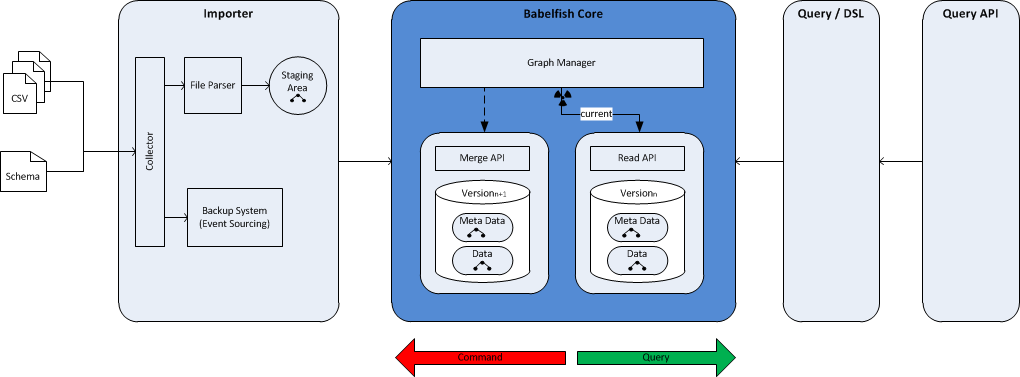
\includegraphics[width=\textwidth]{./graphics/Architecture}
\caption{System Architecture Overview}
\label{fig:Architecture}
\end{figure}
\todo replace Architecture.png by up-to-date picture


\Cref{fig:Architecture} shows an overview of the system architecture. The system is partitioned into three main modules: Core, DSL and Web.

\subsection{Core Module}
The Core module consists of three submodules: Infrastructure, Importer and Schema.

\subsubsection{Infrastructure}
The Infrastructure submodule contains all the code relevant for database access.
This also includes the mapping of the high-level data model to its database representation and the representation of versions on the database level.
Furthermore, the infrastructure code contains configuration- and migration-specific code.
All the other modules use this code to abstract from direct database access.
\subsubsection{Importer}
The Importer is responsible for reading data from CSV format and converting them into graph format.
\subsubsection{Schema}
The Schema module contains an abstract definition of a schema as well as information about cardinalities and type mappings to the Neo4j context.

\subsection{DSL Module}
Babelfish's DSL module consists of a DSL interpreter, a set of core DSL libraries and a set of table-specific DSL functionalities.
The core libraries contain functionality for basic path traversal.
The table-specific functionalities allow for SQL post-processing.

Note that the DSL code can be used to create customized language extensions -- one can then configure the DSL interpreter to make the language extensions available to Babelfish.

\subsection{Web Module}
System access via REST API is provided by the Web module.
It uses the Scalatra Framework to load the various servlet.
Currently, there exist servlets for
\begin{itemize}
\item query execution and job management,
\item node and edge access,
\item schema information,
\item access to log messages and
\item information about the system status and the system's capabilites.
\end{itemize}

as well as a demo browser client, written in HTML and JavaScript.


\section{Tools and Frameworks}
Table \ref{tab:tools} lists the tools and frameworks used during the Babelfish development.
We recommend using the same set of tools and frameworks in order to ensure a trouble-free development process.
\begin{table}[hp]
\begin{tabularx}{\textwidth}{llX}
\toprule
Tool or Framework & Version(s) & References \& Documentation\\
\midrule
Oracle JDK & 7 / 8 & \href{http://www.oracle.com/technetwork/java/javase/downloads/index.html}{Oracle's Java SE Download Page} \\
IntelliJ IDEA & 12 / 13 & \href{http://www.jetbrains.com/idea/download/index.html}{Jetbrains Download Page}\\
\Gls{SBT} & 0.13 & \href{http://www.scala-sbt.org/}{Scala SBT Documentation}\\
\bottomrule
\end{tabularx}
\caption{Tools and Frameworks}\label{tab:tools}
\end{table}

Additionally the IntelliJ plugins in \cref{tab:plugins} were used for a convenient development workflow.

\begin{table}[hp]
\begin{tabularx}{\textwidth}{lX}
\toprule
Plugin & References \& Documentation\\
\midrule
Git & By default bundled with IDE\\
Scala & \href{http://confluence.jetbrains.com/display/SCA/Scala+Plugin+for+IntelliJ+IDEA}{Scala Plugin Documentation}\\
\Gls{SBT} & \href{https://github.com/orfjackal/idea-sbt-plugin/wiki}{SBT Plugin Documentation}\\
\bottomrule
\end{tabularx}
\caption{IntelliJ Plugins}\label{tab:plugins}
\end{table}

\subsection{SBT}
\Gls{SBT} is a build and dependency management tool. For a selection of the most common command see \cref{tab:sbtCommands}.
All commands can be prefixed by \code{\~} to use triggered execution (i.e. commands will be executed whenever a file change occurs).

\begin{table}[hp]
\begin{tabularx}{\textwidth}{llX}
\toprule
Command & Project & Description\\
\midrule
compile & all & Compile code\\
test:compile & all & Compile code including tests\\
test & all & Execute tests\\
set-dev & BF & Set development environment (*.dev.xml)\\
set-prod & BF & Set production environment (*.prod.xml)\\
container:start & BF & Start standalone web server\\
container:stop & BF & Stop standalone web server\\
container:reload /& BF & Restart standalone web server\\
publish-local & BF & Deploy program to ivy cache\\
package-war	& BF & Create Babelfish WAR package (e.g. for Tomcat)\\
jacoco:cover & BF & Create Jacoco test coverage report\\
dependency-graph & BF & Create ASCII graph of 3rd-party dependencies\\
dependency-dot & BF & Create GraphViz DOT of 3rd-party dependencies\\
dependency-license-info & BF & List 3rd-party libraries, sorted by licence\\
package & C & Create BabelfishConfiguration.jar\\
\bottomrule
\end{tabularx}
\caption{SBT Commands}\label{tab:sbtCommands}
\end{table}

\chapter{Deployment}\label{sec:deployment}
\section{Architecture}
\begin{figure}[htbp]
\centering
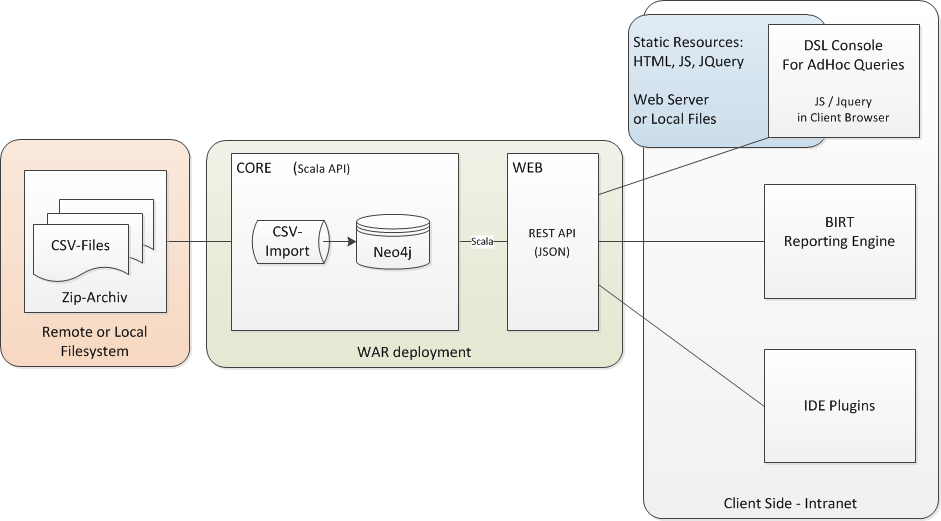
\includegraphics[width=\textwidth]{./graphics/DeploymentOverview}
\caption{Deployment Overview for the Babelfish System}
\label{fig:DeploymentOverview}
\end{figure}
Figure \ref{fig:DeploymentOverview} gives a coarse overview of the Babelfish deployment.
Note that the importer reads from the file system where incoming data is regularly provided as zipped CSV files.
The various intranet clients access the deployed Babelfish system via a uniform REST API.

\subsection{Web service}\label{sec:web}
\todo

\section{System requirements}
Minimal system requirements are very small, for real world scenarios everything depends on speed / space requirements of imports and queries. \Cref{tbl:sysReq} lists the typical development / small database configuration.

\warn[RAM]{Transaction logs of imports and migrations MUST fit within the available RAM. Importing 400k nodes made up of a Long, a DateTime, two short and a longer String requires at least 8GB RAM.}
\info[Import]{Babelfish automatically creates a single transaction for every schema element.}

\begin{table}[H]
\begin{tabularx}{\textwidth}{lX}
\toprule
Hardware \\
\midrule
RAM & > 4GB, depending on data size (recommended >> 8GB) \\
CPU &  current midrange, at least 2-core \\
Storage & local disk/flash storage, size depends on data and archiving needs (the war-file is \~40MB, database will soon be > 2GB)\\
\midrule
Software \\
\midrule
OS & tested on Linux (Ubuntu, Suse), Mac OS X, MS Windows 7 and 8\\
JVM & tested on Oracle JVM 7, 64bit\\
Application server & tested on Tomcat 7 and Jetty 8 \\
\bottomrule
\end{tabularx}
\caption{System requirements}\label{tbl:sysReq}
\end{table}

\chapter{Usage}\label{sec:usage}
A ready to use instance (for deployment see \cref{sec:deployment}) of Babelfish will present a web page including a query form for DSL queries, schema information and statistics information. All information can also be accessed via JSON (\cref{sec:web}).

\section{Configuration}\label{sec:config} \todo

\lstinputlisting[caption={Example configuration}]{examples/src/main/scala/ch/fhnw/imvs/babelfish/BabelfishConfiguration.scala}

\section{Schema}\label{sec:schema} \todo

\section{Import}\label{sec:import} \todo
\att{Import files must be encoded in UTF-8 without BOM.}

\subsection{Migration}
\warn[Experimental]{Migration is an experimental, unsupported feature. Try at your own risk.}

There are two means of migration: small, automatic schema migrations (\cref{sec:autoMigration}) and possibly larger ones, involving rewriting data (\cref{sec:manualMigration}). All migrations are transactional and will create a new database version only if there is no exception.

\subsubsection{Automatic migration}\label{sec:autoMigration}
Automatic migration supports the following use-cases:
\begin{itemize}
\item Adding non-id edges to the schema
\item Adding nodes (possibly with new id edges) to the schema
\item Adding properties to the schema (with a default value for existing elements)
\item Removing non-id properties from the schema
\end{itemize}

To conduct an automatic migration, copy the new \code{BabelfishConfiguration.jar} (\cref{sec:config}) into the \code{import} folder. In order to add new properties to existing elements, \code{def default(p: SchemaElement\#SchemaProperty[_]): Any} must be overridden in the configuration.

\subsubsection{Manual migration}\label{sec:manualMigration}
Manual migration supports the following use-cases:
\begin{itemize}
\item Removing nodes (from the schema)
\item Removing edges (from the schema)
\item Removing id-properties from the schema
\item Renaming nodes and edges
\item Creating and updating nodes and edges
\item All of the automatic ones (\cref{sec:autoMigration})
\end{itemize}

To execute a manual migration implement a function \code{MigrationAPI => Unit} and override \code{def lowlevelMigration: Option[MigrationAPI => Unit]} in the configuration. Then package the configuration and name it \code{Migration.jar}. Copy this jar into the \code{import} directory.

\section{DSL}\label{sec:dsl}
All DSL related code resides in \code{ch.fhnw.imvs.babelfish.dsl}.

\info{A DSL query is basically a so-called traverser:}
\begin{lstlisting}
class Tr[I,O,+A] extends (Env => I => Stream[(O,A)])
\end{lstlisting}
I.e. a function which -- given an \code{Env}ironment -- returns a function from \code{I} to a stream of \code{O,A} tuples. Many traversers have an even more complex form that allows to track paths (the nodes and edges visited), cycles and labels (named values):
\begin{lstlisting}
Tr[State[I],State[O],A]
\end{lstlisting}

Think of these as functions that turn an input state \code{State[I]} (e.g. an edge) into an output state \code{State[O]} (e.g. a node) and yield an arbitrary result \code{A}, e.g. versioned property values.

Traversers may then be combined using combinators (\cref{sec:combinators}).

\detail{\subsection{Primitives}The most basic traversers (\cref{tab:primitives}) are building blocks for higher-level DSL statements and rarely used directly.}
\begin{table}[hp]
\begin{tabularx}{\textwidth}{>{\ttfamily}lX}
\toprule
Traverser & Description\\
\midrule
success[S,A](a):Tr[S,S,A] & returns its input as the output \\
fail[S]:Tr[S,S,Nothing] & drops its input and returns an empty output \\
getEnv[S]:Tr[S,S,QueryDb] & returns the QueryDb (graph database API) \\
getState[S]:Tr[S,S,S] & returns the current state \\
setState[I,O](o:O):Tr[I,O,Unit] & sets the current state\\
\bottomrule
\end{tabularx}
\caption{Primitive traversers}\label{tab:primitives}
\end{table}

\subsection{Navigation}
Navigation traversers allow to move within the graph.
\begin{table}[hp]
\begin{tabularx}{\textwidth}{>{\ttfamily}lX}
\toprule
Traverser & Description \\
\midrule
V(sn:SchemaNode) & all nodes of type \code{sn}\\
E(se:SchemaEdge) & all edges of type \code{se}\\
outE(se:SchemaEdge) & the outgoing edges of type \code{se} of the current path's head node\\
inE(se:SchemaEdge) & the incoming edges of type \code{se} of the current path's head node\\
outV() & the source vertex of the current path's head edge\\
inV() & the target vertex of the current path's head edge\\
out(se:SchemaEdge) & \code{outE(se) \~> inV()}\\
in(se:SchemaEdge) & \code{inE(se) \~> outV()}\\
\bottomrule
\end{tabularx}
\caption{Navigation traversers}\label{tab:navTrav}
\end{table}

Additionally there are traversers (\cref{tab:valTrav}) to retrieve property values and the path visited so far.

\begin{table}[hp]
\begin{tabularx}{\textwidth}{>{\ttfamily}lX}
\toprule
Traverser & Description \\
\midrule
get(p:SchemaProperty) & retrieve the property \code{p} of the current path head\\
path() & the current path\\
versions() & the versions of the path head\\
\bottomrule
\end{tabularx}
\caption{Value traversers}\label{tab:valTrav}
\end{table}

\subsection{Filtering, Matching and Sub-Queries}
Filter traversers retain only paths whose head values satisfy a given predicate. Similarly, matching allows to take different actions depending on whether or not paths accord with a given pattern. Sub-queries allow branching without modification of the outer context. These traversers are listed in \cref{tab:filterTrav}. For a detailed description of the versioning aspect see \cref{sec:versioning}.

\begin{table}[hp]
\begin{tabularx}{\textwidth}{>{\ttfamily}lX}
\toprule
Traverser & Description \\
\midrule
tr.filter(p:A=>Boolean) & only keep paths where \code{p(a) == true}\\
tr.filterV(p:A=>Boolean) & restrict the current path to versions where the value of the head \code{Versioned[A]} satisfies \code{p} (if empty discard the path)\\
\multicolumn{2}{l}{\code{where(sp:SchemaProperty[A])(p:A=>Boolean)}\hspace{2\tabcolsep} get(sp).filterV(p)}\\
sub(tr) & continue with \code{tr}'s result, without modifying the state\\
tr.matches(p:Tr) & a traverser indicating whether \code{tr\~p} is non-empty\\
\bottomrule
\end{tabularx}
\caption{Filter traversers}\label{tab:filterTrav}
\end{table}


\subsection{Combinators}\label{sec:combinators}
Combinators are used to create powerful traversers by combining simpler ones. All traversers that take part in a combination must obey certain rules. The \code{*} combinator for example only accepts traversers that start and end on the same type. \Cref{tab:comboSemantics,tab:comboSyntax} lists these combinators.

\begin{table}[hp]
\begin{tabularx}{\textwidth}{>{\ttfamily}lX}
\toprule
Syntax & Description \\
\midrule
t1 <\~> t2 & sequential composition of traversers \code{t1} and \code{t2} \\
t1 | t2 &  choice (parallel composition) of traversers \code{t1} and \code{t2} \\
t >> ft & context-sensitive traversal (feed result of \code{t} to \code{ft} or lookup next traverser.) \\
t \^ \^ f & transform the result of \code{t} with function \code{f} \\
t.? & make \code{t} optional, result will be without and (if possible) with \code{t} \\
t.+ & follow \code{t} at least once (result will contain no cycles, see \cref{sec:cycle}) \\
t.* & follow \code{t} zero or more times (see also \cref{sec:cycle})\\
\midrule
t1 <\~ t2 & like \code{<\~>} but only keep track of \code{t1}\\
t1 \~ t2 & like \code{<\~>} but only keep track of \code{t2}, default for performance reasons\\
t1 \~> t2 & like \code{<\~>} but only keep track of \code{t2}\\
\bottomrule
\end{tabularx}
\caption{Combinator semantics}\label{tab:comboSemantics}
\end{table}

\begin{table}[hp]
\begin{tabularx}{\textwidth}{>{\ttfamily}l>{\ttfamily}X}
\toprule
Syntax & Traverser (St = State) \\
\midrule
t1 <\~> t2 & seq[I,O,P,A,B](t1:Tr[I,O,A], t2:Tr[O,P,B]): Tr[I,P,A<\~>B]\\
t1 | t2 & choice[I,O,A](t1:Tr[I,O,A], t2: =>Tr[I,O,A]): Tr[I,O,A] \\
t >> ft & t.flatMap[P,B](ft:A=>Tr[O,P,B]): Tr[I,P,B]\\
t \^ \^ f & t.map[B](f:A=>B): Tr[I,O,B]\\
t.? & opt[S,A](t:Tr[S,S,A]): Tr[S,S,Option[A]]\\
t.+ & many1[E,A](tr:Tr[St[E],St[E],A]):Tr[St[E],St[E],Stream[A]]\\
t.* & many[E,A](tr:Tr[St[E],St[E],A]): Tr[St[E],St[E],Stream[A]]\\
\midrule
t1 <\~ t2 & (t1 <\~> t2).map\{ case a <\~> b => a \}\\
t1 \~ t2 & t1 \~> t2\\
t1 \~> t2 & (t1 <\~> t2).map\{ case a <\~> b => b \}\\
\bottomrule
\end{tabularx}
\caption{Combinator syntax}\label{tab:comboSyntax}
\end{table}


\subsubsection{Cycle detection}\label{sec:cycle}
When running a graph traverser containing a repetition (\code{.+} or \code{.*}), there are two ways to run into cycles: 
Either the graph data itself contains cyclic structures or the traverser generates a cycle on a non-cyclic structure (as in \code{(outE(X) \~ outV()).+}).
To avoid endless cycling in these situations, the DSL repetition functionality automatically detects slices that were already traversed and ignores paths that contain a slice more than once.


\subsection{Versioning}\label{sec:versioning}
For each traversed path, the versions it is valid for are tracked. Initially the versions are set to the versions of the first element. Then, each traversal step further restricts the versions by intersecting with the versions of the traversed elements. If a path's version becomes empty, this signifies that there is no single version where the whole path is valid, and the path is therefore discarded.

Furthermore, we can work with versions using the traversers in \cref{tab:versionTraversers}.
\begin{table}[hp]
\begin{tabularx}{\textwidth}{>{\ttfamily}lX}
\toprule
Traverser & Description \\
\midrule
tr.added & version in which the element matched by \code{tr} was first added\\
tr.removed & version in which the element matched by \code{tr} was last removed (or \code{HEAD}, if it was never removed)\\
tr.addedAfter(v:Version) & elements where \code{added > v}\\
tr.addedBefore(v:Version) & elements where \code{added < v}\\
tr.intersect(vrs:VersionRangeSet) & intersect current version with \code{vrs} (and limit the current path head's version accordingly)\\
\bottomrule
\end{tabularx}
\caption{Version-related traversers}\label{tab:versionTraversers}
\end{table}


\subsection{Extraction and Post-Processing}
\subsubsection{Labels}
Labels can be assigned and filtered by using the \code{as}-syntax:
\begin{table}[H]
\begin{tabularx}{\textwidth}{>{\ttfamily}lX}
\toprule
Syntax & Description \\
\midrule
t.as("X") & assign the label \code{X} to traverser \code{t}.\\
t.sameAs("X") & filter for paths where traverser \code{t} was previously assigned label \code{X}.\\
\bottomrule
\end{tabularx}
\caption{As-syntax}\label{tab:asSyntax}
\end{table}


\subsubsection{Extraction to Table Format}
Labelled traversers can be extracted to table format using the \code{from}-syntax:

\begin{lstlisting}
from (t1.as("X")).extract()
\end{lstlisting}

The \code{extract} functionality can only be applied to a \code{from}-block, which can contain a traverser with an arbitrary number of labels.
If \code{extract} is called without arguments, the extracted table contains all the assigned labels from the \code{from}-block.
Alternatively, one can limit the variables to extract as follows:

\begin{lstlisting}
from (t1.as("X1") \~ t2.as("X2") \~ t3.as("X3")).extract ("X1", "X2")
\end{lstlisting}

\detail[Flattening of Versions for Table Output]{Extracted properties will usually be versioned and can therefore contain different values.
In order to obtain a regular table format, these versioned properties are flattened in such a way that every column contains exactly one value.
The associated versions are added to the end of the table as the columns \code{VERSION.FROM} and \code{VERSION.TO}.}

\subsubsection{Semi-automatic labeling and extraction}
For utmost convenience there are two traversers that label and extract data at the same time:
\begin{table}[H]
\begin{tabularx}{\textwidth}{>{\ttfamily}lX}
\toprule
Syntax & Description \\
\midrule
ex(p: SchemaProperty, prefix = "") & \code{get(p).as(prefix + p.name)} \\
exAll(prefix = "") & Extract and label all properties of the most recent SchemaElement head \\
\bottomrule
\end{tabularx}
\caption{Ex traversers}\label{tab:ex}
\end{table}

\subsubsection{SQL Post-Processing}
After extracting a result as a table, we can optionally post-process it using SQL queries.
Within the SQL query, the table can be referred to as \code{t1}. Each column is named according to its name in the table, whereby all occurrences of "." are replaced by "_" for SQL compatibility.
A DSL query using SQL post-processing might look as follows:

\begin{lstlisting}
from(V(X).as("X1")).extract().sql("select X1, VERSION_FROM from t1")
\end{lstlisting}

\detail[In-Memory SQL Processor]{The SQL processor uses an HSQL in-memory database. For detailed documentation on its features, see \url{http://hsqldb.org/}.}


\subsection{Partial result sets and ordering}
\Cref{tab:misc} lists operations used for sorting and computing only as many results as needed. \info[Order and Scope]{\code{tr.ascending.take(1)} returns the path with the smallest result value (and must therefore first compute all possible results) whereas \code{tr.take(1).ascending()} sorts a stream of one (arbitrary) result. \code{tr1 \~ tr2.take(1)} will execute \code{tr2} for each result of \code{tr1} and take each first result of \code{tr2}, \code{(tr1 \~ tr2).take(1)} will execute \code{tr2} at most once and yields at most one result.}

\begin{table}[hp]
\begin{tabularx}{\textwidth}{>{\ttfamily}lX}
\toprule
Traverser & Description \\
\midrule
tr.take(n:Int) & only compute the first \code{n} paths\\
tr.ascending() & order paths ascending by result value\\
tr.descending() & order paths descending by result value\\
\bottomrule
\end{tabularx}
\caption{Misc traversers}\label{tab:misc}
\end{table}

\subsection{Syntax}
DSL queries may be formulated according to the constructions in \cref{fig:DSLquery}. To keep the diagrams simple all bracketing is omitted. Scala's rules apply.

\begin{figure}[hp]
\begin{grammar}

<TrailsQuery> ::= \[[\begin{stack}<traverser>\\ <from> \begin{stack}<extract>\begin{stack}<sql>\\\end{stack}\\\end{stack}\end{stack}\]]

<traverser> ::= \[[\begin{stack}`V(' node `)'\\`E(' edge `)'\end{stack} \begin{rep}\begin{stack}\\<trOp>\end{stack}\begin{stack}<tie> <tr>\\\end{stack}\end{rep}\]]

<tie> ::= \[[\begin{stack}\begin{stack}\\`<'\end{stack}`~'\begin{stack}\\`>'\end{stack}\\`|'\end{stack}\]]

<tr> ::= \[[\begin{stack}
`V(' node `)'\\`E(' edge `)'\\
`in(' edge `)'\\`out(' edge `)'\\`inE(' edge `)'\\`outE(' edge `)'\\
`ex(' property \begin{stack}\\`,' string\end{stack} `)' \\`exAll('\begin{stack}\\string\end{stack}`)'\\`get(' property `)'\\
`sub(' <tr> `)'\\`matches(' <tr> `)'\\`matchesNot(' <tr> `)'\\`where('property`)('propertyType => Boolean`)'\\
`path()'\\`versions()'\\
`added()'\\`removed()'\\`addedAfter(' version `)'\\`removedAfter(' version `)'\\
`intersect(' versionRangeSet `)'\end{stack}\]]

<trOp> ::= \[[`.'\begin{stack}`?'\\`+'\\`*'\\`as(' string `)'\\`take(' number `)'\\`map(' lastResType => newResType `)'\\`filter(' lastResType => Boolean `)'\\`filterV(' lastResType => Boolean `)'\\`ascending'\\`descending'\end{stack}\]]

\end{grammar}
\caption{The (simplified) grammar of DSL queries}\label{fig:DSLquery}
\end{figure}

\begin{figure}[hp]
\ContinuedFloat
\begin{grammar}
<from> ::= \[[`from {' <traverser> `}'\]]

<extract> ::= \[[`extract {' \begin{stack}\\\begin{rep} string\\ `,' \end{rep}\end{stack}`}'\]]

<sql> ::= \[[`sql {' \begin{stack}<sqlStatement>\\\end{stack}`}'\]]

<sqlStatement> ::= \[[ "sql statement selecting from `t1'" \]]
\end{grammar}
\caption[]{The (simplified) grammar of DSL queries}
\end{figure}

\subsection{Extensions} \todo

\subsection{Query Performance}
To discuss query performance, we want to take into account all the involved stages of a query execution:
\begin{itemize}
\item Query transmission to the Babelfish server
\item Compilation
\item Execution on the graph database
\item Potentially: Table Extraction and SQL processing
\item Presentation of the result
\item Result transmission from the server to the client
\item Result presentation at the client site (typically: in the browser)
\end{itemize}

Let's address the phases in order:
\paragraph{Query transmission to the server and Compilation} are usually very fast and almost never a performance issue.

\paragraph{Execution on the graph database} can take a lot of time, depending mainly on the amount of data that is traversed in order to obtain the result.
If we want to obtain very large results, this may be unavoidable.
If, on the other hand, the expected result is considerably smaller than the amount of traversed data, we might be able to reduce execution time.
\info[Tips to reduce Query Execution Time]{
\begin{itemize}
\item "Strongest filter first": If one part of the query contains a strong filter, try to place it first. E.g. the query\\
\code{V(Company) \~ out(_Employees_) \~ where(Person.Name)(_\ == "Peter")}\\
can probably be optimized by reformulating to:\\
\code{V(Person) \~ where(Person.Name)(_\ == "Peter") \~ in(_Employees_)}
\item Know the magnitude of the data, and start your query with the less numerous.\\
\code{V(Country) \~ out(_Inhabitants_)}\\
will most likely be faster than\\
\code{V(People) \~ in(_Inhabitants_)}
\item If you don't need the complete result set, limit it using \code{take}:\\
\code{V(People).take(100)}
\end{itemize}
}
Note that query execution is likely to be significantly faster when the query is run a second time due to caching of the graph database.

\paragraph{Table Extraction and SQL Processing} usually takes time proportional to the result size.
SQL processing can, of course, take longer time for more complex SQL queries.

\paragraph{Presentation of the result, result transmission to the client and result presentation} often comprises a relatively large part of the overall duration.
It does, however, usually take time proportional to the result size.
Therefore, the most effective way to reduce this time component is to think about the required result:
Do we really need the whole results, or can we aggregate or even omit some parts?
\todo review / complete

\info[Query Timings]{The Babelfish server measures the duration of the phases compilation, execution, extraction, sql processing and presentation to complete. These timings are part of the query result (the demo browser client displays them at the bottom of each result).}

\detail[Browser Performance]{For very large results, it happens that the browser exhibits performance issues or crashes entirely while the Babelfish system still works fine.
It might help to disable memory-intensive result rendering or, possibly, try doing it with another browser.}

\section{REST API}
The rest API is structured into four parts:
\begin{enumerate}
\item Job management (\cref{tab:RESTJobs})
\item Schema information (\cref{tab:RESTSchema})
\item Direct querying of schema elements (\cref{tab:RESTDirectData})
\item Logs and other data (\cref{tab:RESTMisc})
\end{enumerate}

\info[REST Data Format]{Throughout the Babelfish API, the default data format is JSON. The client can change this to Xml by setting the content type to "application/xml" or to toString-serialised Scala objects by setting content type "text/plain". When mentioned, additional content types can be requested by providing a url suffix. This is usually the case for more complex content, e.g. query results in pdf format.}

\begin{table}[hp]
\begin{tabularx}{\textwidth}{XlX}
\toprule
URL & HTTP Method & Functionality \\
\midrule
/bf/jobs/ & GET & Forward to /bf/jobs/list\\
/bf/jobs/list & GET & List all jobs (job id, query string, starting and end time, result type, status)\\
/bf/jobs/execute/\{query\} & POST & Start new job with query string \code{query}, return new job id\\
/bf/jobs/cancel/\{jobId\} & DELETE & Abort job \code{jobId}, delete its result\\
/bf/jobs/cancel_all & DELETE & Abort all jobs, delete all results\\
/bf/jobs/count/active & GET & Number of running jobs\\
/bf/jobs/count/all & GET & Total number of jobs\\
/bf/jobs/results/\{jobId[.suffix]\}\newline[?aggregated=true|false\&layout=dot|sfdp] & GET & Result of job \code{jobId} (as soon as it is ready). Optionally, a suffix (.pdf, .svg, .xml, .gv or .csv) can be given. With aggregation edges between nodes are weighted and drawn only once, for the layout parameter see the GraphViz documentation.\\
\midrule
/bf/jobs/execute/\{query\} & GET & Deprecated\\
/bf/jobs/cancel/\{jobId\} & GET & Deprecated\\
/bf/jobs/cancel_all & GET & Deprecated\\
\bottomrule
\end{tabularx}
\caption{REST Functionality: Job Management}\label{tab:RESTJobs}
\end{table}

\begin{table}[hp]
\begin{tabularx}{\textwidth}{llX}
\toprule
URL & HTTP Method & Functionality\\
\midrule
/bf/schema/[\{name\}.]\{suffix\} & GET & Schema with \code{name} in \code{suffix} format. If \code{name} is omitted, the currently active schema is used. Supported formats are: .pdf, .svg, .xml, .gv\\
/bf/schema/csv & GET & Schema in CSV format\\
/bf/schema/meta & GET & Information about the schema\\
/bf/schema/graph & GET & All schema nodes and edges\\
/bf/schema/nodes & GET & All schema nodes\\
/bf/schema/nodes/\{nodeName\} & GET & Schema node with \code{nodeName}\\
/bf/schema/edges & GET & All schema edges\\
/bf/schema/edges/\{edgeName\} & GET & Schema edge with \code{edgeName}\\
\bottomrule
\end{tabularx}
\caption{REST Functionality: Schema Information}\label{tab:RESTSchema}
\end{table}

\begin{table}[hp]
\begin{tabularx}{\textwidth}{llX}
\toprule
URL & HTTP Method & Functionality\\
\midrule
/bf/nodes/\{id\} & GET & Node by \code{id}\\
/bf/edges/\{id\} & GET & Edge by \code{id}\\
\bottomrule
\end{tabularx}
\caption{REST Functionality: Direct Data Retrieval}\label{tab:RESTDirectData}
\end{table}

\begin{table}[hp]
\begin{tabularx}{\textwidth}{llX}
\toprule
URL & HTTP Method & Functionality\\
\midrule
/bf/log & GET & List all log messages\\
/bf/log/\{x\}-\{y\} & GET & List log messages \code{x} to \code{y}\\
/bf/log/count & GET & Number of log messages\\
capabilities/dot & GET & Show (boolean) dot capabilities of the server.\\
\bottomrule
\end{tabularx}
\caption{REST Functionality: Misc}\label{tab:RESTMisc}
\end{table}

\section{Examples}
\info[All examples are based on Carol’s world (\cref{fig:carol}).]{Please consult the accompanying project for example code.}
\subsection{Schema}
Carol’s domain consists of persons and their pets. Each person is identified by their name, a pet is identified by its name and and its owner. (see \cref{lst:CarolSchema})

\begin{figure}[hp]
\noindent\resizebox{\linewidth}{!}{
\begin{tikzpicture}[->,>=stealth',node distance=2cm,nodes={ellipse,fill=black!10,draw,minimum height=.75cm,minimum width=2cm}]
 \node (a) {Alice};
 \node (b) [right = of a] {Bob};
 \node (c) [below = 2cm of a] {Carol};
 \node (d) [right = of c] {Dave};
 \node[rectangle] (m) [right = of b] {Murphy};
 \node[rectangle] (f) [right = of d] {Fluffy};

  \path[every node/.style={font=\sffamily\small}]
  (a) edge [bend left] node[auto,swap] {loves} (b)
  (a) edge node[auto] {likes} (c)
  (b) edge [bend left] node[auto,swap] {loves} (a)
  (m) edge[thick] node[auto] {owner} (b)
  (c) edge node[auto,swap] {loves} (b)
  (c) edge node[auto] {likes} (d)
  (f) edge[thick] node[auto] {owner} (d)
  ;
\end{tikzpicture}}
\caption{Carol’s world}\label{fig:carol}
\end{figure}

\subsubsection{Importer}
\chapter{Known Issues, Limitations, Future Work}
\begin{itemize}
\item Cardinalities are not enforced
\item Interpreter security (use dedicated security manager, reset `garbage' of last user)
\item Migration discards all diff information (causes full import for all elements on next import), could be more fine-granular.
\item Current database is forcefully stopped once a new version is ready. May cause exceptions in active jobs.
\item Temporal consistency is not enforced, e.g. it is allowed to create an active edge to an inactive node or to deactivate nodes without deactivating adjacent edges. 
\end{itemize}

%==========
\backmatter
\chapter{Appendix}
\section {Code}
\lstinputlisting[caption={Schema for Carol's World},label={lst:CarolSchema}]{examples/src/main/scala/ch/fhnw/imvs/babelfish/example/CarolSchema.scala}

\printglossary[style=altlist]
\listoftables
\listoffigures
\lstlistoflistings
%\bibliography{...}
%\printindex

\end{document}
